
The following describes the classes and subclasses used to create the ontology in Protege.
\\

\begin{itemize}
    \item \textbf{Classes} (that are subclasses of owl:Thing):
    \begin{itemize}
        \item Organism;

        \item Habitat;

        \item Resource.
        \\
    \end{itemize}

    \item \textbf{Subclasses}:
    \begin{itemize}
        \item Animal, Plant and Microorganism as subclasses of Organim (all mutually disjoint from each other);

        \item Herbivore and Carnivore as subclasses of Animals (they are both disjoint);

        \item Bryophytes and  Angiosperms as subclasses of Plants (all mutually disjoint from each other).
        \\
    \end{itemize} 
\end{itemize}

It is important to note that all classes and subclasses are mutually exclusive; therefore, no individual from one class can belong to another, and no individual from one subclass can belong to another subclass. The hierarchy of classes can be better observed in the figure below.

\begin{figure}[H]
    \centering
    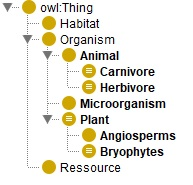
\includegraphics[width=0.35\linewidth]{images/ontology/classes.jpg}
    \caption{Class hierarchy}
    \label{fig:diagram}
\end{figure}


Regarding the Class properties, we have the following \textbf{Data properties}:
\\

    \begin{itemize}
        \item \textit{weight} with domain Animal and range xsd:decimal;

        \item \textit{has\_Fruits} with domain Angiosperms and range xsd:boolean;

        \item \textit{chemical\_formula} with domain Ressource and range xsd:string. We set this property to be unique, as it will be used as the identifier of the ressource;

        \item \textit{geographical\_coordinates} with domain Habitat and range xsd:string. It also has the unique property, and will be used as the identifier of the environment;

        \item \textit{scientific\_name} with domain Organism and range xsd:string. Again, it's unique and used as an indentifier for the organisms.
        \\

    \end{itemize}


The following two figures illustrate both the declaration of data properties and the method used to ensure the uniqueness of the \textit{scientific\_name}, for example.
\\

\begin{figure}[H]
    \centering
    \begin{minipage}{0.35\textwidth}
        \centering
        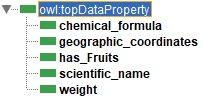
\includegraphics[width=\textwidth]{images/ontology/mini1.jpg}
        \caption{Data properties}
        \label{fig:figura1}
    \end{minipage}%
    \hspace{0.1\textwidth}
    \begin{minipage}{0.35\textwidth}
        \centering
        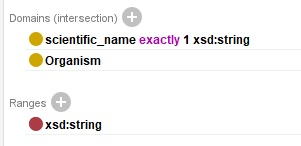
\includegraphics[width=\textwidth]{images/ontology/mini2.jpg}
        \caption{Unique property}
        \label{fig:figura2}
    \end{minipage}
\end{figure}

Finally, we have the following \textbf{Object properties}:
\\

    \begin{itemize}
        \item \textit{eat} with domain Animal and range Animal $\cup$ Plant;

        \item \textit{livesIn} with domain Organism and range Habitat;

        \item \textit{consumeTheResource} with domain Organism and range Resource;

        \item \textit{isEatenBy} with domain Organism and range Animal (is the inverse property \textit{eat});

        \item \textit{isOccupiedBy} with domain Habitat and range Organism (is the inverse of \textit{livesAt});

        \item \textit{hasTheResource} with domain Habitat and range Resource;

        \item \textit{isInTheEnvironment} with domain Resource and range Habitat (inverse of the property \textit{hasTheResource})

        \item \textit{coExistWith} with domain Organism and range Organism. This property is symmetric. In addition, this property is different if both organisms are animals/plants or if they are both microorganisms:
        \begin{enumerate}
            \item $A$ and $B$ are animals/plants: \textit{A} coexists with \textit{B} means that \textit{A} and \textit{B} lives at the same environment (livesIn(A) == livesIn(B)) \textbf{and} they do not share neither the relation \textit{A} isEatenBy \textit{B} nor \textit{B} isEatenBy \textit{A};

            \item $A$ and $B$ are both microorganisms: \textit{A} coexists with \textit{B} means that \textit{A} and \textit{B} lives at the same environment (livesIn(A) == livesIn(B)) \textbf{and} they do not consume the same resource through the relation consumeTheResource;
            \\
            
        \end{enumerate}
    \end{itemize}

The list of object properties in Protege can be seen in the figure below.

\begin{figure}[H]
    \centering
    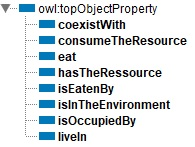
\includegraphics[width=0.35\linewidth]{images/ontology/obg_protp.jpg}
    \caption{Object properties}
    \label{fig:diagram}
\end{figure}

The inference rules were described using \textit{SWRL} (Semantic Web Rule Language), which allows for writing it in a practical and concise manner. Below, we provide a detailed description of all the inference rules related to object and data properties.
\\

We start by the following inference rule: if Organism $a$ eat Organism $b$, and Organism $a$ live in the Habit $env$, then $b$ should also live in $env$. This is described by:
\\

\begin{lstlisting}
eat(?a, ?b) ^ liveIn(?a, ?env) -> liveIn(?b, ?env)
\end{lstlisting}


The same way, if Organism $a$ coexists with Organism $b$, and $a$ live in the Habitat $env$, $b$ should also live in $env$.
\\

\begin{lstlisting}
coexistWith(?a, ?b) ^ liveIn(?a, ?env) -> liveIn(?b, ?env)
\end{lstlisting}

Now, regarding the plants, we can infer that a plant is an angiosperm if it has a fruit, which is a binary variable. Therefore, we have the following rule:
\\

\begin{lstlisting}
has_Fruits(?a, true) -> Angiosperms(?a)
\end{lstlisting}

From now on, we will focus on discussing the coexistence relationship, which is the most complex relation of the ontology. As previously described, according to our rules, a carnivorous animal will always coexist with another carnivorous animal as long as they inhabit the same environment. Additionally, we add the rule that animal $a$ must be different from $b$, as we do not want the relation to be reflexive. To ensure that they are both different, we require that their scientific names be different, using the syntax \textit{differentFrom}.
\\

\begin{lstlisting}
Carnivore(?a) ^ Carnivore(?b) ^ liveIn(?a, ?env) ^ liveIn(?b, ?env) ^ scientific_name(?a, ?name_a) ^ scientific_name(?b, ?name_b) ^ differentFrom(?name_a, ?name_b) -> coexistWith(?a, ?b)
\end{lstlisting}

We use the same logic to describe the coexistence for the herbivores, as follows:
\\

\begin{lstlisting}
Herbivore(?a) ^ Herbivore(?b) ^ liveIn(?a, ?env) ^ liveIn(?b, ?env) ^ scientific_name(?a, ?name_a) ^ scientific_name(?b, ?name_b) ^ differentFrom(?name_a, ?name_b) -> coexistWith(?a, ?b)
\end{lstlisting}

Also, carnivorous animals will always coexist with the plants that inhabit the same environment. In this case, it's enough to add the proposition \textit{differentFrom(?a, ?b)} because if $a$ is a Carnivore (by the previous proposition) and $b$ is a Plant (also stated earlier), they should be different because both classes are disjoint.
\\

\begin{lstlisting}
Carnivore(?a) ^ Plant(?b) ^ liveIn(?a, ?env) ^ liveIn(?b, ?env) ^ differentFrom(?a, ?b) -> coexistWith(?a, ?b)
\end{lstlisting}

Next, we have the case of coexistence between plants, which is similar to the herbivore's case:
\\


\begin{lstlisting}
Plant(?a) ^ Plant(?b) ^ liveIn(?a, ?env) ^ liveIn(?b, ?env) ^ scientific_name(?a, ?name_a) ^ scientific_name(?b, ?name_b) ^ differentFrom(?name_a, ?name_b) -> coexistWith(?a, ?b)
\end{lstlisting}

Finally, the coexistence between two microorganism happens when they both live in the same environment \textbf{and} do not consume the same resource. To guarantee that both resources are different, we use again their unique identifier, which is the \textit{chemical\_formula}:
\\

\begin{lstlisting}
Microorganism(?a) ^ Microorganism(?b) ^ consumeTheResource(?a, ?res_a) ^ consumeTheResource(?b, ?res_b) ^ liveIn(?a, ?env) ^ liveIn(?b, ?env) ^chemical_formula(?res_a, ?formula_a) ^ chemical_formula(?res_b, ?formula_b) ^ differentFrom(?formula_a, ?formula_b) ^ scientific_name(?a, ?name_a) ^ scientific_name(?b, ?name_b) ^ differentFrom(?name_a, ?name_b) -> coexistWith(?a, ?b)
\end{lstlisting}
